% ============================================================================
% MathNLP 2026 submission — anonymous review copy
% Symbolic vs LLM graders for multi-step math derivations
% ----------------------------------------------------------------------------
% BUILD SETUP:
%   The ACL style files (acl.sty, acl_natbib.bst) are already included in this
%   directory. No local TeX install is required if you build on Overleaf: just
%   upload this folder, or start from Overleaf's "ACL" template and drop in the
%   sections/ and refs.bib. Locally:
%       pdflatex main ; bibtex main ; pdflatex main ; pdflatex main
%
% Submit in REVIEW mode (anonymous). Flip to the camera-ready option only after
% acceptance. Long paper = 8 pages of content (refs/appendices excluded).
% ============================================================================
\documentclass[11pt]{article}

% For submission (anonymous, line numbers):
\usepackage[review]{acl}
% For camera-ready, replace the line above with:  \usepackage[]{acl}

\usepackage{times}
\usepackage{latexsym}
\usepackage[T1]{fontenc}
\usepackage[utf8]{inputenc}
\usepackage{microtype}
\usepackage{booktabs}
\usepackage{graphicx}
\usepackage{amsmath}
\usepackage{amssymb}
\usepackage{multirow}

\title{What Symbolic Graders Can't See and {LLM} Judges Won't Ignore:
Abstention-Aware Comparison of Step-Level Math Graders}

% Name is set here; \usepackage[review]{acl} still prints "Anonymous ACL
% submission" on the PDF until camera-ready (\usepackage{acl}).
\author{Anirudh Balaji}

\begin{document}
\maketitle

\begin{abstract}
Automatic grading of multi-step mathematical derivations is a prerequisite for
evaluating math-capable retrieval-augmented and reasoning systems, yet the two
dominant graders, symbolic equivalence checkers and LLM-as-judge, are rarely
compared under a single, reproducible protocol. We present such a comparison on
derivations produced by a retrieval-augmented assistant over a
signals-and-systems corpus. We evaluate a SymPy-based symbolic verifier against
two LLM judges from independent labs (\texttt{gpt-oss-120b}, open-weight;
\texttt{claude-sonnet-4-5}, proprietary) on two labeled testbeds: a
human-labeled ground-truth set over the assistant's own derivations for 29
benchmark queries (191 steps, 13 error steps), and a controlled synthetic
error-injection suite over 9 hand-authored gold derivations (14 mutations across
5 families). The
symbolic verifier is high-precision but high-abstention on both testbeds: on
the injection suite, precision $1.00$, false-positive rate $0.00$, strict
recall $0.234$, abstention $0.64$; on the human set, abstention $0.53$ and
strict recall $0.000$ on all 13 human-flagged errors, of which $9/13$ lie
outside the symbolic fragment and $4/13$ are in-fragment misses (human-set
precision/recall measure agreement with a rubric the judges were not shown),
whereas LLM judges achieve near-total coverage and higher agreement on those
labels, at the cost of injection-suite false positives concentrated on
equivalence-preserving rewrites (FPR $8.7$--$18.2\%$). The
\emph{qualitative} pattern is model-independent across both judges, but the exact
precision/recall operating point is model-dependent (judge--judge $\kappa{=}0.31$
on committed steps; the two judges catch overlapping but distinct human errors). Paired McNemar tests with Holm--Bonferroni
correction ($n{=}191$; six tests) confirm the coverage and recall gaps
($p_{\mathrm{Holm}}{<}0.05$). A symbolic$\rightarrow$LLM cascade improves the
injection trade-off (e.g.\ cascade$\rightarrow$\texttt{claude}: recall $0.904$,
FPR $0.042$) but can reduce human-set recall when symbolic false passes lock out
the judge; thresholding the judge's own confidence yields precision--coverage
curves that make abstention an explicit dial. Labels are single-annotator; we mitigate by releasing
the rubric and all raw labels. We argue that grader choice is a
precision/coverage trade-off rather than a correctness question, that the
obvious cascade should be measured rather than assumed, and that
math-NLP evaluations should report \emph{abstention rates} alongside pass/fail.
We release code, prompts, the open-weight judge configuration, all labels, and
frozen results at \url{https://osf.io/5kvqe/?view_only=8c0032bd76244a1daaebf6cb3feb2c92}.

\end{abstract}

\section{Introduction}
\label{sec:intro}

Large language models increasingly produce \emph{multi-step} mathematical
derivations, not only final answers, inside retrieval-augmented generation
(RAG) and tool-using reasoning systems. Evaluating those systems therefore
requires grading intermediate steps, not just checking a boxed result. There is
no consensus on how to do that grading. Two families dominate practice.
\emph{Symbolic} verifiers compare a predicted expression to a reference with a
computer-algebra system and are exact on the fragment they can parse.
\emph{LLM-as-judge} graders prompt a second model to accept, reject, or abstain
on a step and apply far more broadly. Both are widely used; they are almost never
compared head-to-head under one protocol that treats abstention as a first-class
outcome. Practitioners therefore lack clear guidance on which grader to trust,
when, and what error modes each hides.

We address this gap with a reproducible comparison of a SymPy-based symbolic
verifier against two LLM judges from independent labs:
\texttt{gpt-oss-120b} (open-weight) and \texttt{claude-sonnet-4-5} (proprietary).
All graders score the same steps under a shared covered/abstain accounting, on
two labeled testbeds: a 29-query human-labeled set (191 steps) drawn from the
derivations of a RAG assistant over a signals-and-systems corpus, and a
controlled synthetic error-injection suite over 9 hand-authored gold
derivations. Our central finding
is that the choice is not ``which grader is
correct,'' but a \emph{precision versus coverage} trade-off. The symbolic
verifier is high-precision and high-abstention: it rarely false-alarms where it
commits, but it abstains often and misses all 13 real human-flagged errors in
this domain, which lie overwhelmingly outside the symbolic fragment. LLM
judges achieve near-total coverage and catch many of those errors, at the cost
of injection-suite false positives concentrated on equivalence-preserving
rewrites. The \emph{qualitative} pattern holds across both
judges; the exact precision/recall operating point does not
(\texttt{claude} is more aggressive, \texttt{gpt-oss} more conservative).

\paragraph{Contributions.}
\begin{itemize}
    \item A single reproducible protocol that scores a symbolic verifier and two
    LLM judges on the \emph{same} covered/abstain split, over two labeled
    testbeds: a 29-query human-labeled ground-truth set and a synthetic
    error-injection suite (14 mutations, 5 families, 9 gold derivations), with
    paired step-level significance tests
    (\S\ref{sec:setup}--\S\ref{sec:protocol}).
    \item A three-way empirical comparison showing symbolic
    high-precision/high-abstention versus LLM near-total coverage with higher
    false-positive rate, with exact McNemar tests and Holm--Bonferroni
    correction on $n{=}191$ steps (\S\ref{sec:results}).
    \item An evaluated \emph{cascade} policy (symbolic first, LLM judge on
    abstain) that improves the injection precision/FPR trade-off but can
    \emph{hurt} human-set recall when symbolic false passes lock out the judge
    (\S\ref{sec:cascade}), plus precision--coverage curves from thresholding
    the judge's unused confidence field (\S\ref{sec:confidence}).
    \item A cross-judge robustness result: the qualitative trade-off holds across
    an open-weight and a proprietary judge, while the operating point is
    model-dependent (\S\ref{sec:analysis}).
    \item An open, rerunnable release, including the open-weight judge
    configuration so reviewers can reproduce that grader exactly, together with
    prompts, the labeling rubric, all human labels, and frozen verdicts/tables
    at \url{https://osf.io/5kvqe/?view_only=8c0032bd76244a1daaebf6cb3feb2c92}.
\end{itemize}

\section{Related Work}
\label{sec:related}

\paragraph{Symbolic and formal verification of mathematics.}
Computer-algebra systems such as SymPy \citep{meurer2017sympy} support exact
symbolic equivalence checking and are widely used as lightweight verifiers for
mathematical expressions. A complementary line of work aims at
\emph{formal} verification via proof assistants and autoformalization, translating
natural-language mathematics into machine-checkable statements
\citep{wu2022autoformalization}. These approaches are sound where they apply,
but they are limited to the fragment that can be parsed, formalized, or proven.
Our symbolic grader sits in the lightweight CAS regime: fast and exact on
covered steps, silent or inapplicable elsewhere.

\paragraph{LLM-as-judge and its failure modes.}
Using a strong LLM to grade another model's output is now a standard evaluation
tool \citep{zheng2023judging,liu2023geval}. Documented failure modes include
positional and other fairness biases \citep{wang2024faireval}, self-preference
for an evaluator's own generations \citep{panickssery2024selfpref}, and brittle
agreement with humans under adversarial or carefully curated pairs
\citep{zeng2024llmbar,thakur2025judging}. We study a related but distinct
failure in the math setting: judges that over-flag \emph{equivalence-preserving}
rewrites as errors, even when a symbolic checker correctly accepts them. By
running two judges from independent labs under one prompt and metric suite, we
separate model-independent patterns from model-specific operating points, and
reduce (though do not eliminate) the risk that a single judge's self-preference
dominates the comparison \citep{panickssery2024selfpref}.

\paragraph{Evaluating mathematical reasoning and locating errors.}
Math benchmarks such as GSM8K \citep{cobbe2021gsm8k} and MATH
\citep{hendrycks2021math} typically score final answers. Process-level
supervision and step-wise reward models push evaluation toward intermediate
reasoning \citep{uesato2022process,lightman2024verify,wang2024mathshepherd}.
Complementary \emph{step-quality} suites score chains for validity,
informativeness, or embedding-based consistency
\citep{golovneva2023roscoe,prasad2023receval,xia2025reasoneval}; ReasonEval in
particular evaluates error detection under perturbation, closest in spirit to
our injection suite \citep{xia2025reasoneval}. Meta-reasoning benchmarks such as
{MR-GSM8K} ask models to locate and explain mistakes in solutions
\citep{zeng2025mrgsm8k}. Closest to our human-set findings, \citet{tyen2024errors}
show that LLMs struggle to \emph{find} reasoning
errors even when they can \emph{correct} them given the error location: the
same bottleneck our judges hit on real, mostly out-of-fragment mistakes (F1) and
over-flagging of surface edits (F2). Rather than proposing a new grader or
benchmark, we evaluate two existing graders directly, scoring a symbolic
verifier and two LLM judges on the same multi-step derivations under one
protocol.

\paragraph{Abstention and selective prediction.}
Our framing, coverage vs.\ precision with abstention as a first-class
outcome, follows the tradition of reject options and selective
classification \citep{chow1970reject,elyaniv2010selective,geifman2017selective}
and its NLP instantiation as selective question answering
\citep{kamath2020selective}. We treat symbolic \textsc{none} and
confidence-thresholded judge abstention as two concrete reject policies for
math grading, and report coverage/precision trade-offs rather than forced
pass/fail alone.

\paragraph{Answer equivalence.}
Token-level match underestimates true answer quality when paraphrases and
semantically equivalent forms are treated as errors
\citep{bulian2022tomayto}. Our F2 finding is the process-level analogue:
equivalence-preserving algebraic rewrites are correct under a CAS checker but
often flagged by LLM judges.

\section{Setup}
\label{sec:setup}

\subsection{Task and corpus}
We study step-level grading of mathematical derivations produced by a
retrieval-augmented \citep{lewis2020rag} assistant over a single fixed corpus in
signals and systems. The generator that produced the frozen derivations is
\texttt{qwen-3-235b-a22b-instruct-2507} served via the Cerebras OpenAI-compatible
API (temperature $0$), as recorded in the schema-v2 envelope of the release
eval run. That model ID has since been withdrawn by the provider (HTTP 404);
we therefore treat the derivation set as a fixed artifact and do not regenerate
it under a replacement model.
Each query has a structured expected answer, and the assistant emits an ordered
list of steps, each a symbolic expression together with a short natural-language
description of the operation performed. A grader inspects one step at a time,
given the question and all prior steps as context, and returns one of
\textsc{passed}, \textsc{failed}, or \textsc{abstain}. We map these to
$\{\textsc{true}, \textsc{false}, \textsc{none}\}$ so that every grader is scored
on an identical covered/abstain split (\S\ref{sec:protocol}).

Our benchmark contains 30 queries and is the \emph{source} of the graded
derivation traces, not a separate evaluation set. One query (Q12) failed during
generation and has no label template, so all human-labeled results use the
remaining 29 queries; we report this as a known gap rather than silently
dropping it. Of those 29, 27 come from the primary frozen generator run and two
(Q01, Q07) from an earlier run with the same model ID and temperature $0$; the
released label templates are the ground truth for all grading tables.

\subsection{Symbolic verifier}
The symbolic verifier uses SymPy \citep{meurer2017sympy} to test equivalence
between a step and the derivation context, with additional matchers for composite
expressions and inequalities. By construction it commits only when it can
establish or refute equivalence and abstains otherwise; it therefore never
``guesses.''

\subsection{LLM judges}
The LLM judge is a swappable client selected by environment variables, so a new
judge model flows through the entire pipeline without code changes. Each judge
receives a fixed rubric and step template (reproduced in
Appendix~\ref{app:prompt}) and returns a verdict, a confidence, and a short
rationale. We evaluate two judges chosen from \emph{independent} labs so the
paper can test whether findings are model-specific:
\texttt{gpt-oss-120b} \citep{openai2025gptoss}, an open-weight reasoning model, and
\texttt{claude-sonnet-4-5}, a proprietary model. Using an open-weight judge is a
deliberate reproducibility choice: a reviewer can run the exact grader.

\subsection{Error-injection suite}
To obtain controlled ground truth, we programmatically mutate \emph{9
hand-authored gold derivations} (standard signals/algebra results such as the
Laplace and Fourier transforms of $e^{-at}u(t)$, partial fractions, and the
time-shift property) with 14 mutation operators grouped into five families. The
gold derivations are independent of the generator and verified to pass the
symbolic checker unmutated, so any flag on a mutated step is attributable to the
mutation rather than to a mislabeled baseline. Three families
inject genuine errors: \emph{algebraic} (e.g.\ sign flips), \emph{bounds}
(integration-limit errors), and \emph{identifier} (variable-identity errors).
Two families are negatives that a grader should \emph{not} flag:
\emph{control} (no-op) and \emph{equivalent} (equivalence-preserving rewrites).
This lets us measure both recall on real errors and false positives on
legitimate reformulations. The 9 gold derivations contain 14 mutable step
sites in total; every mutation operator is attempted against every site, for
$14 \times 14 = 196$ attempted (step $\times$ mutation) trials. Of these,
78 are skipped because the mutation does not apply to that step's expression;
the graded suite is the remaining 118 trials (94 error, 24 non-error:
14 control $+$ 10 equivalent).

\section{Evaluation Protocol}
\label{sec:protocol}

\paragraph{Testbeds.}
We evaluate graders on \emph{two} labeled testbeds. (i)~The
\textbf{human-labeled} set: assistant-generated derivations for the 29 usable
queries of our 30-query benchmark (one query, Q12, has no usable derivation;
\S\ref{sec:setup}), in which a human annotator marked each step
\textsc{correct}/\textsc{incorrect} and, for incorrect steps, an error type. It
contains 191 steps, of which 13 are human-flagged errors (missing\_term $=6$,
definition $=4$, algebra $=3$). (ii)~The \textbf{error-injection} suite of
\S\ref{sec:setup}: programmatic mutations of 9 hand-authored gold derivations,
where the label is defined by the mutation rather than by an annotator. The
benchmark is the source of the traces in (i), not a separate evaluation set, and
the injection suite is deliberately independent of the generator so that
detection is measured against known-correct baselines.

\paragraph{Human labeling rubric vs.\ judge prompt.}
The human labels follow an explicit annotation rubric that includes a
\emph{notation-strictness} rule: a step is marked incorrect if boundary or
integration-by-parts notation is written wrong, or if a claimed equation is
incomplete, even when the underlying algebra would evaluate correctly. The LLM
judges never see this rubric. They receive only the step prompt in
Appendix~\ref{app:prompt}, which asks whether the stated operation, applied to
the previous expression, produces the current expression: a purely local
mathematical-validity criterion, with no notation-strictness clause. This is a
deliberate mismatch: we evaluate judges as typically deployed (generic step
prompt), not as annotators trained on our rubric. Consequently, on the human
set, precision and recall are \emph{not} measures of ``correctness'' against an
oracle the judge was instructed to match. They measure \textbf{agreement with a
rubric the judge did not see}. Disagreements can therefore reflect either a
genuine math miss or a policy gap (e.g., the human failing a notationally
incomplete but algebraically harmless step that the judge accepts). Injection
metrics are unaffected: error labels there are defined by the mutation, not by
the human rubric.

\paragraph{Metrics.}
Treating ``the step is wrong'' as the positive class, we use \textbf{one}
definition on every row of every table. On committed (non-abstain) predictions:
\textbf{precision} $=\mathrm{TP}/(\mathrm{TP}+\mathrm{FP})$ and
\textbf{FPR} $=\mathrm{FP}/(\mathrm{FP}+\mathrm{TN})$ (covered negatives only).
\textbf{Recall is strict:}
$\mathrm{TP}/(\mathrm{TP}+\mathrm{FN}+\mathrm{AbsE})$, where AbsE is
abstain (or an unparseable/crash response, counted as abstain) on a true-error case.
Abstaining on an error is therefore a miss, not a silent exclusion from the
denominator. Across all cases we report \textbf{coverage} (committed fraction)
and \textbf{abstain rate}. Confusion cells TP/FP/TN/FN are among committed
verdicts only; AbsE/AbsN make the counts add to $N$. On the human set,
precision/recall are agreement with the unseen human rubric (above); on
injection they are detection metrics against planted mutations. This strict
recall matches the paired \texttt{caught\_error} statistic in
\S\ref{sec:results}.

\paragraph{Shared covered/abstain split.}
All graders are scored with the same routine and the same
$\{\textsc{true},\textsc{false},\textsc{none}\}$ mapping, so differences reflect
grader behavior and not scoring conventions. The LLM judge sees exactly the
\emph{step context} the human annotator saw (question $+$ prior steps), but not
the human's labeling rubric.

\paragraph{Significance testing.}
For the head-to-head on the human set we compare each judge to the symbolic
verifier on the same 191 steps (paired). The three binary outcomes are
\emph{committed} (coverage), \emph{correct\_committed} (committed \emph{and}
matching the human label; abstains score $0$), and \emph{caught\_error} (strict
recall on the 13 error steps). Because these are paired binary indicators, the
primary test is an \emph{exact McNemar} test \citep{mcnemar1947note} on
discordant pairs, following standard guidance for paired binary NLP comparisons
\citep{dror2018hitchhikers}. We also report descriptive $10{,}000$-replicate
bootstrap $95\%$ CIs on the mean delta (judge$-$symbolic) and, for continuity
with earlier drafts, a sign-flip permutation $p$. With two judges $\times$ three
metrics we have a family of six tests; we control the family-wise error rate with
Holm--Bonferroni \citep{holm1979simple} at $\alpha{=}0.05$, following
\citep{dror2018hitchhikers}. Bootstrap CIs
for \texttt{caught\_error} use only $n{=}13$ error steps and are treated as
\emph{uninformative} when they hit a $\{0,1\}$ boundary (we do not quote them to
three decimals).

\section{Results}
\label{sec:results}

\subsection{Headline three-way comparison}
Table~\ref{tab:threeway} and Figure~\ref{fig:fig1} summarize every grader on
both labeled testbeds under a single metric definition
(\S\ref{sec:protocol}): \emph{strict} recall (abstain-on-error counts as a miss)
and FPR among covered negatives. The pattern is consistent. The symbolic
verifier commits on only $47.1\%$ of human-labeled steps and $35.6\%$ of
injection trials; where it commits it is essentially never wrong (injection
precision $1.00$, FPR $0.00$), but its strict recall is $0.000$ on the 13 human
errors and only $0.234$ on injected errors. Both LLM judges instead commit
almost everywhere (coverage $\geq 0.92$) and agree with far more of the human
error labels (strict recall $0.462$ for \texttt{gpt-oss} and $0.769$ for
\texttt{claude}; injection recall $0.851$ and $0.904$), but they pay for it in
false positives, with injection FPR $0.087$ and $0.182$ respectively, while the
symbolic verifier's FPR stays at $0$. These injection FPR values rest on few
covered negatives (20, 23, and 22 covered non-errors out of 24 total, for
symbolic, \texttt{gpt-oss}, and \texttt{claude}); the
\texttt{gpt-oss}--\texttt{claude} gap is 2 vs.\ 4 false positives, and $95\%$
Wilson intervals are wide and overlapping ($[0.024, 0.268]$ vs.\ $[0.073,
0.385]$), so the FPR ordering is directional rather than precisely estimated.
Human-set precision/recall are agreement
with a rubric the judges did not see (\S\ref{sec:protocol}).

\begin{table*}[t]
\centering
\footnotesize
\setlength{\tabcolsep}{2.8pt}
\begin{tabular}{llrrrrrrrrrr}
\toprule
dataset & grader & cov. & prec. & rec. & FPR & abst. & TP & FP & TN & FN & AbsE \\
\midrule
\multirow{3}{*}{human}
 & symbolic & 0.471 & n/a & 0.000 & 0.000 & 0.529 & 0 & 0 & 83 & 7 & 6 \\
 & \texttt{gpt-oss-120b} & 0.995 & 0.667 & 0.462 & 0.017 & 0.005 & 6 & 3 & 175 & 6 & 1 \\
 & \texttt{claude-sonnet-4-5} & 0.953 & 0.370 & 0.769 & 0.100 & 0.047 & 10 & 17 & 153 & 2 & 1 \\
\midrule
\multirow{3}{*}{injection}
 & symbolic & 0.356 & 1.000 & 0.234 & 0.000 & 0.644 & 22 & 0 & 20 & 0 & 72 \\
 & \texttt{gpt-oss-120b} & 0.941 & 0.976 & 0.851 & 0.087 & 0.059 & 80 & 2 & 21 & 8 & 6 \\
 & \texttt{claude-sonnet-4-5} & 0.924 & 0.955 & 0.904 & 0.182 & 0.076 & 85 & 4 & 18 & 2 & 7 \\
\bottomrule
\end{tabular}
\caption{Three-way grader comparison on the human-labeled ($n{=}191$ steps; 13
errors) and error-injection ($n{=}118$ applicable trials; 94 errors, 24
non-errors) testbeds. \textbf{One definition throughout:} coverage $=$ committed
fraction; precision $=\mathrm{TP}/(\mathrm{TP}+\mathrm{FP})$; \emph{strict}
recall $=\mathrm{TP}/(\mathrm{TP}+\mathrm{FN}+\mathrm{AbsE})$ (abstain-on-error
is a miss); FPR $=\mathrm{FP}/(\mathrm{FP}+\mathrm{TN})$ on covered negatives.
TP/FP/TN/FN are among committed verdicts only; AbsE $=$ abstain or
unparseable/crash on a true-error case. Identity:
$\mathrm{TP}+\mathrm{FP}+\mathrm{TN}+\mathrm{FN}+\mathrm{AbsE}+\mathrm{AbsN}=n$
(AbsN omitted for space; see \texttt{threeway\_table.json}). On the human set,
precision/recall measure agreement with the human rubric the LLM judges were
not shown (\S\ref{sec:protocol}). Human-set recall denominators are all 13
errors, matching Table~\ref{tab:paired}.}
\label{tab:threeway}
\end{table*}

\begin{figure}[t]
\centering
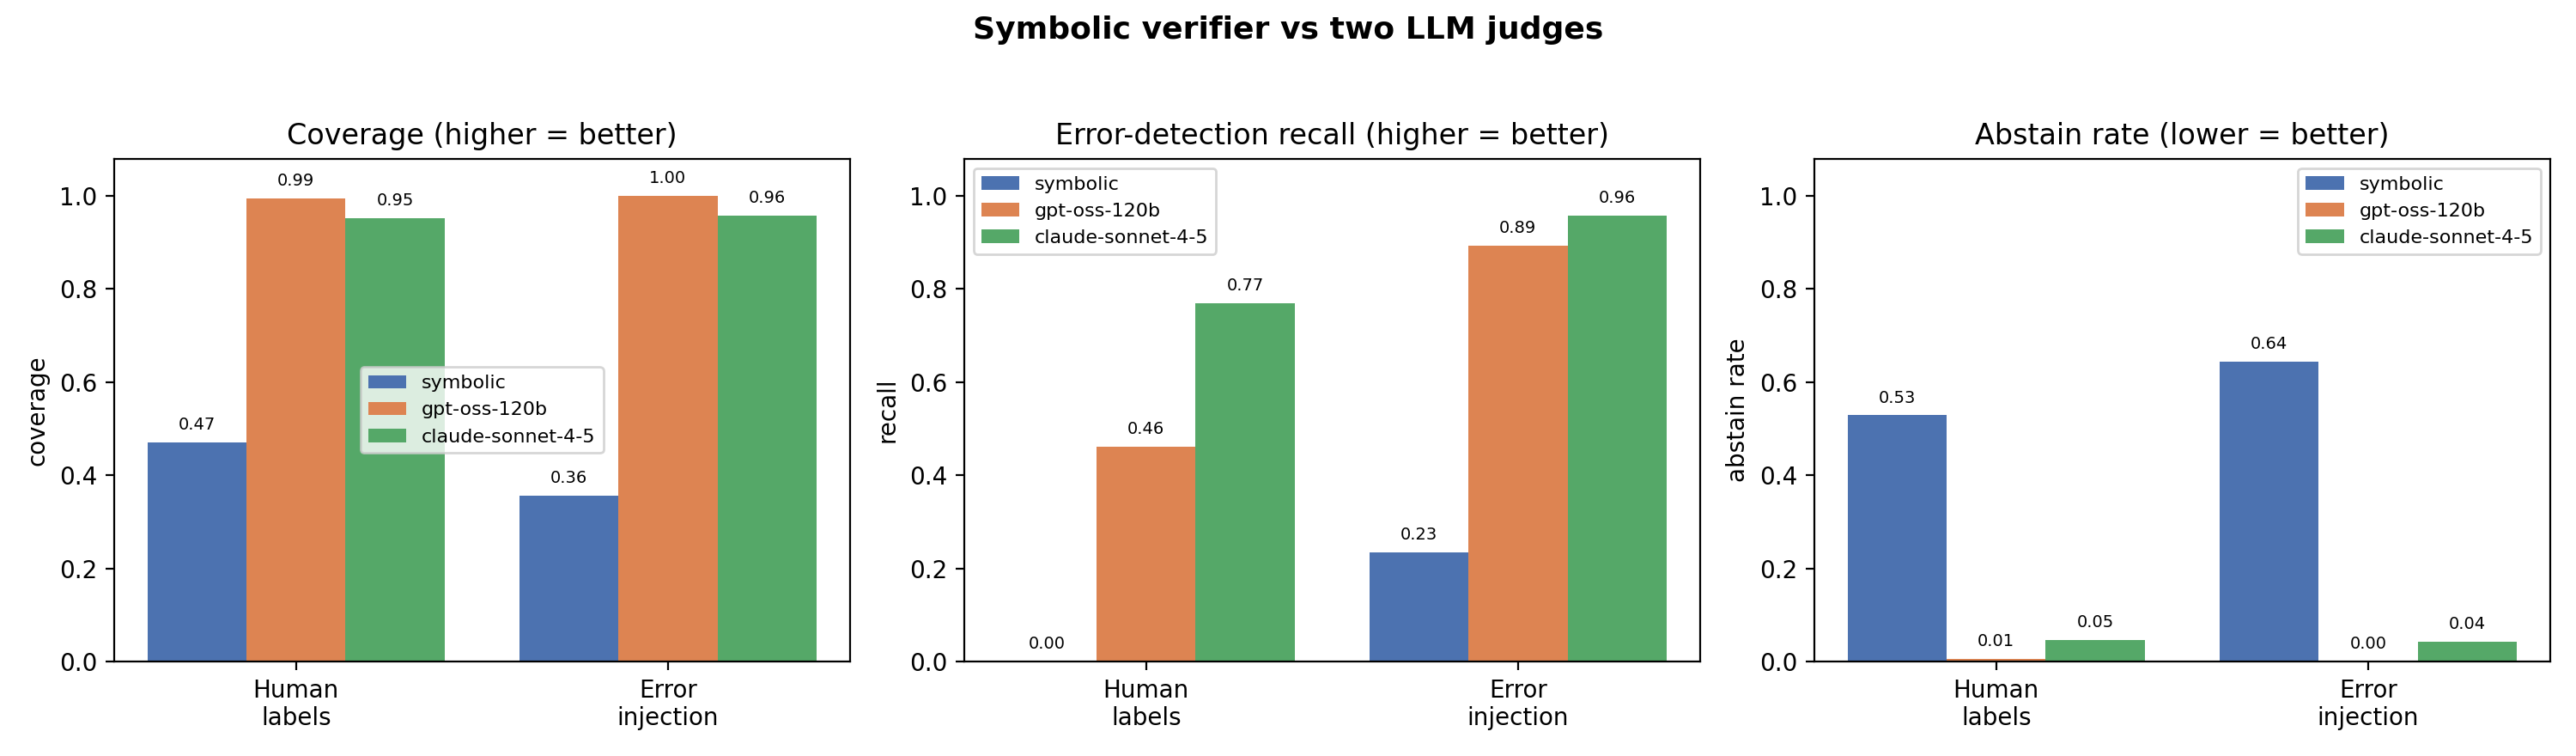
\includegraphics[width=\columnwidth]{../results/figures/fig1_grader_comparison.png}
\caption{Coverage, strict error-detection recall, and abstention for the three
graders on both testbeds. Symbolic trades coverage for zero false positives; the
LLM judges do the opposite.}
\label{fig:fig1}
\end{figure}

\subsection{Paired significance on the human set}
Table~\ref{tab:paired} reports the paired step-level comparison of each judge
against the symbolic verifier on the same 191 steps. Exact McNemar tests with
Holm--Bonferroni correction over the six-test family
\citep{dror2018hitchhikers} reject the null for all six comparisons at
$\alpha{=}0.05$: both judges have higher coverage and
correct\_committed rates than symbolic ($p_{\mathrm{Holm}}\!\ll\!0.001$), and
higher strict recall on the 13 error steps
($p_{\mathrm{Holm}}{=}0.031$ for \texttt{gpt-oss}, $0.0039$ for
\texttt{claude}). Point estimates match Table~\ref{tab:threeway}
($\Delta_{\mathrm{caught}}{=}{+}0.46$ and ${+}0.77$). Bootstrap CIs for
\texttt{caught\_error} are omitted as uninformative ($n{=}13$; Claude's would
reach the boundary $1$; Limitations).

\begin{table}[t]
\centering
\small
\resizebox{\columnwidth}{!}{%
\begin{tabular}{llrll}
\toprule
judge & metric & $\Delta$ & 95\% CI & McNemar $p$ / Holm $p$ \\
\midrule
\multirow{3}{*}{\texttt{gpt-oss}}
 & committed          & $+0.524$ & $[0.450, 0.592]$ & $<\!10^{-20}$ / $<\!10^{-20}$ \\
 & correct\_committed & $+0.513$ & $[0.440, 0.586]$ & $<\!10^{-20}$ / $<\!10^{-20}$ \\
 & caught\_error      & $+0.46$ & uninf.\ ($n{=}13$) & $0.031$ / $0.031$ \\
\midrule
\multirow{3}{*}{\texttt{claude}}
 & committed          & $+0.482$ & $[0.403, 0.560]$ & $<\!10^{-20}$ / $<\!10^{-20}$ \\
 & correct\_committed & $+0.419$ & $[0.335, 0.497]$ & $<\!10^{-17}$ / $<\!10^{-16}$ \\
 & caught\_error      & $+0.77$ & uninf.\ ($n{=}13$; hits 1) & $0.0020$ / $0.0039$ \\
\bottomrule
\end{tabular}%
}
\caption{Paired step-level differences (judge $-$ symbolic). Primary test:
exact McNemar on discordant pairs; Holm--Bonferroni over six tests
($\alpha{=}0.05$). Bootstrap CIs are descriptive where shown; omitted for
\texttt{caught\_error} ($n{=}13$; uninformative, since Claude's interval would
reach 1).}
\label{tab:paired}
\end{table}

\subsection{Cascade: symbolic first, judge on abstain}
\label{sec:cascade}

Run the symbolic verifier first and invoke an LLM judge only when it abstains.
We evaluate that cascade
\emph{post hoc} on the frozen verdicts (no new model calls) against all three
standalone graders (Table~\ref{tab:cascade}). The rule is fixed: if symbolic
commits, take its verdict; else take the judge; else abstain. Metrics match
Table~\ref{tab:threeway}.

\begin{table*}[t]
\centering
\footnotesize
\setlength{\tabcolsep}{2.5pt}
\begin{tabular}{llrrrrrr}
\toprule
dataset & grader & cov. & prec. & rec. & FPR & abst. & (sym / judge / abs) \\
\midrule
\multirow{5}{*}{human}
 & symbolic & 0.471 & n/a & 0.000 & 0.000 & 0.529 & --- \\
 & \texttt{gpt-oss} & 0.995 & 0.667 & 0.462 & 0.017 & 0.005 & --- \\
 & \texttt{claude} & 0.953 & 0.370 & 0.769 & 0.100 & 0.047 & --- \\
 & cascade$\rightarrow$\texttt{gpt-oss} & 0.995 & 0.600 & 0.231 & 0.011 & 0.005 & 90 / 100 / 1 \\
 & cascade$\rightarrow$\texttt{claude} & 0.984 & 0.263 & 0.385 & 0.080 & 0.016 & 90 / 98 / 3 \\
\midrule
\multirow{5}{*}{injection}
 & symbolic & 0.356 & 1.000 & 0.234 & 0.000 & 0.644 & --- \\
 & \texttt{gpt-oss} & 0.941 & 0.976 & 0.851 & 0.087 & 0.059 & --- \\
 & \texttt{claude} & 0.924 & 0.955 & 0.904 & 0.182 & 0.076 & --- \\
 & cascade$\rightarrow$\texttt{gpt-oss} & 0.966 & 0.976 & 0.872 & 0.083 & 0.034 & 42 / 72 / 4 \\
 & cascade$\rightarrow$\texttt{claude} & 0.941 & 0.988 & \textbf{0.904} & \textbf{0.042} & 0.059 & 42 / 69 / 7 \\
\bottomrule
\end{tabular}
\caption{Standalone graders vs.\ the symbolic$\rightarrow$LLM cascade (same
metric definitions as Table~\ref{tab:threeway}). Rightmost column: how many
cascade decisions came from symbolic, from the judge, or remained abstain.
On injection, cascade$\rightarrow$\texttt{claude} keeps Claude's recall while
cutting FPR from $0.182$ to $0.042$; cascade$\rightarrow$\texttt{gpt-oss} raises
recall over the judge alone ($0.851\rightarrow 0.872$) at matched precision. On
the human set both cascades \emph{lose} recall relative to the judge alone,
because the verifier's 7 committed passes on human-error steps (5
mid-derivation false passes, 2 first-step definitional passes;
Table~\ref{tab:human-errors}) are locked in and never reach the judge.}
\label{tab:cascade}
\end{table*}

On the injection suite the cascade is a clear win. Symbolic contributes its
high-precision commits (42/118 trials); the judge covers most abstains. With
\texttt{claude} as the fallback, recall stays at $0.904$ while FPR drops from
$0.182$ to $0.042$ and precision rises to $0.988$, the best injection operating
point in the study. With \texttt{gpt-oss}, recall improves on the judge alone
($0.851\rightarrow 0.872$) at essentially unchanged precision/FPR.

On the human set the same policy backfires on recall. Symbolic commits on
90/191 steps, including all 7 committed passes on human-error steps (5
mid-derivation false passes plus 2 first-step definitional passes;
Table~\ref{tab:human-errors}; Table~\ref{tab:threeway}, FN$=7$). The cascade
trusts those passes, so the judge never sees them:
cascade$\rightarrow$\texttt{gpt-oss} recall falls from $0.462$ to $0.231$, and
cascade$\rightarrow$\texttt{claude} from $0.769$ to $0.385$. Coverage stays high
and FPR edges down, but the errors the verifier is blind to become irreversible
false negatives. This degradation is deterministic given the verifier's
false-pass count, a structural warning about cascade design rather than a
corpus-specific result. The prescription is therefore conditional: \textbf{cascade when
symbolic commits are trustworthy} (algebraic / injection-like regimes);
\textbf{do not let symbolic passes veto the judge} on steps outside the symbolic
fragment (\S\ref{sec:analysis}).

\paragraph{Cost and latency price tag.}
``Use both'' needs a bill. Symbolic verification is local CPU at effectively
$\$0$ ($\approx\!60$\,ms/step, $\approx 11$\,s total on the 191 human steps on
one laptop CPU; absolute timings are machine-dependent), and because it
already commits on the steps it can verify, the cascade cuts LLM calls by
$47\%$ on the human set ($191\!\rightarrow\!101$) and $36\%$ on injection
($118\!\rightarrow\!76$). Estimated dollar costs at published list rates fall
by the same fraction (Appendix~\ref{app:cost}), but rate cards change; the
call-count reduction does not, and any deployment can measure it directly
without our prices.

\subsection{Confidence thresholding: precision--coverage curves}
\label{sec:confidence}

Each LLM judge already returns a confidence in $[0,1]$ with every verdict
(Appendix~\ref{app:prompt}); prior sections ignored it. We recover a family of
operating points \emph{for free} by committing only when
$\mathrm{confidence}\ge\tau$ and abstaining otherwise
(Figure~\ref{fig:fig3}). Coverage is a dial, not a fixed property of the model.

On the human set, raising $\tau$ trades recall for precision. \texttt{gpt-oss}
at $\tau{=}0.95$ moves precision $0.667\!\rightarrow\!0.833$ and FPR
$0.017\!\rightarrow\!0.006$ at coverage $0.927$, but recall falls
$0.462\!\rightarrow\!0.385$. \texttt{claude} at $\tau{=}0.90$ moves precision
$0.370\!\rightarrow\!0.500$ and FPR $0.100\!\rightarrow\!0.026$ at coverage
$0.848$, at a steeper recall cost ($0.769\!\rightarrow\!0.308$) since its
catches concentrate in lower-confidence verdicts. Thresholding is a
false-positive control, not a free improvement, and these are illustrative
in-sample operating points; a deployment would calibrate $\tau$ on held-out
data. On injection, high $\tau$ pushes \texttt{gpt-oss} toward precision $1.0$
(coverage $0.466$ at $\tau{=}0.99$), while \texttt{claude}'s more compressed
confidences give a flatter curve; both move along the same precision/recall
frontier rather than escaping it (complementary to the cascade of
\S\ref{sec:cascade}).

\begin{figure}[t]
\centering
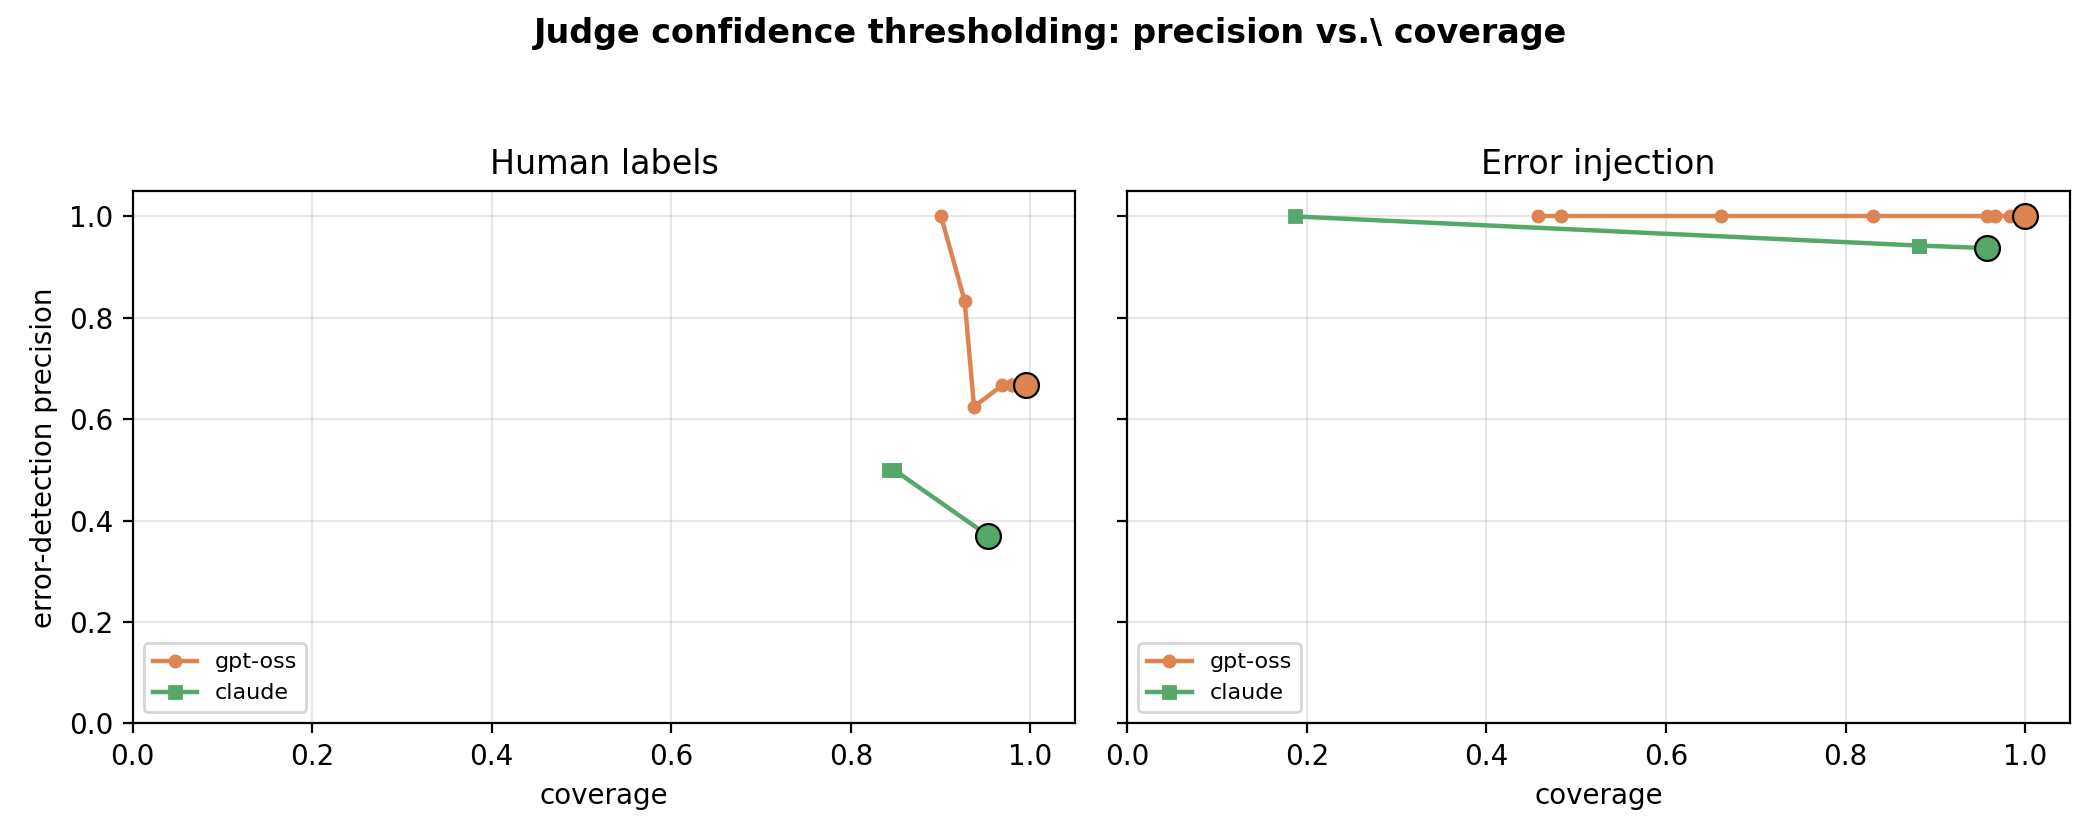
\includegraphics[width=\columnwidth]{../results/figures/fig3_precision_coverage.png}
\caption{Error-detection precision vs.\ coverage under confidence thresholding
(commit iff $\mathrm{confidence}\ge\tau$). Black-edged markers are the default
operating points ($\tau{=}0$) from Table~\ref{tab:threeway}. Curves use only
frozen judge outputs; no new API calls.}
\label{fig:fig3}
\end{figure}

\subsection{Head-to-head and injection families}
Restricting to steps where both \texttt{gpt-oss} and symbolic committed, they
agree and are correct on 82 steps and both wrong on 4; of the 13 human errors,
the judge caught 6 the verifier missed, the verifier caught 0 the judge
missed. The verifier never committed where the judge abstained, and the judge
committed on 100 steps the verifier abstained on, exactly the slice the
cascade routes to it.

Figure~\ref{fig:fig2} breaks the injection suite down by mutation family: as
F1 notes (\S\ref{sec:analysis}), symbolic detects errors only in the algebraic
family, while the judges cover every family but concentrate false positives
on equivalence-preserving rewrites (F2).

\begin{figure}[t]
\centering
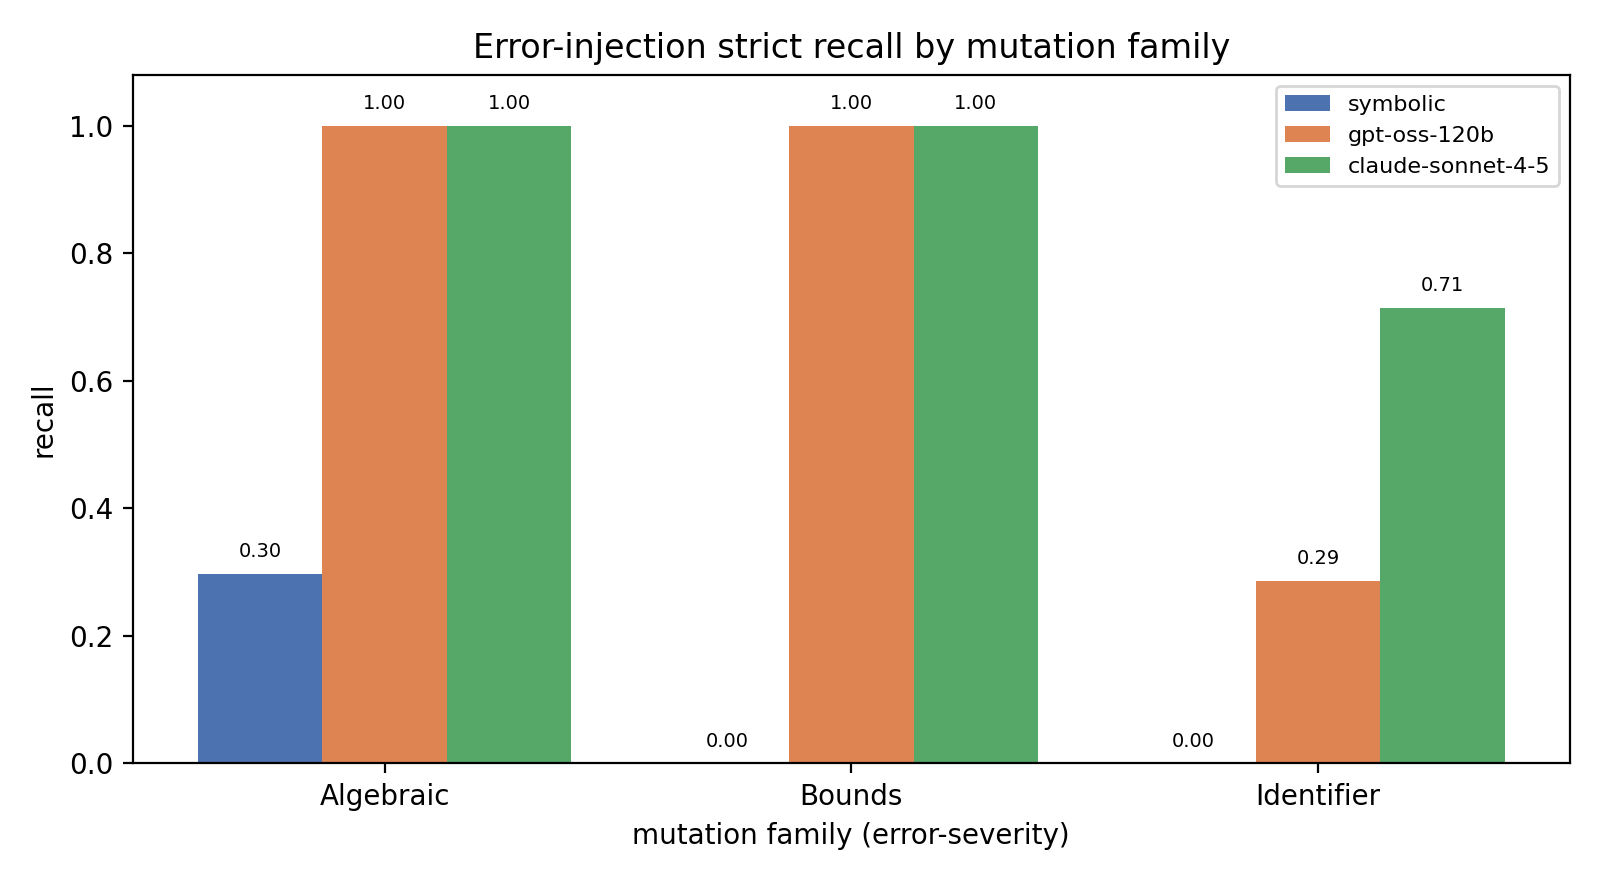
\includegraphics[width=\columnwidth]{../results/figures/fig2_injection_by_family.png}
\caption{Per-family \emph{strict} recall on the injection suite (error-severity
families only: $n{=}74$ algebraic, $6$ bounds, $14$ identifier graded trials).
Symbolic recall is $0.00$ on bounds and identifier (full abstention); nonzero
detection is confined to algebraic mutations. LLM judges cover all families.}
\label{fig:fig2}
\end{figure}

\section{Analysis: Where Each Grader Fails}
\label{sec:analysis}

\paragraph{F1: Real errors are mostly outside the symbolic fragment.}
The verifier's $0.000$ recall on the human set is not a fluke of sample size.
We manually classify each of the 13 human-flagged errors as
\emph{in-fragment} if an ideal CAS step checker, testing algebraic equivalence
of the written expression against a correct continuation of the prior math, could
in principle refute it, and \emph{out-of-fragment} otherwise (definitional
convention, wrong problem setup, property claims relative to an intended target,
or notation/completeness failures under a strict presentation rubric where the
written fragment remains algebraically consistent with a correct outcome).
Full per-step labels appear in Appendix~\ref{app:human-errors}.

\textbf{9 of 13 errors ($69\%$) are out-of-fragment}: real human-flagged
mistakes in this domain are overwhelmingly outside what symbolic equivalence
can see, including wrong Laplace conventions, inconsistent signal definitions,
incomplete equations under notation-strict labeling, and missing boundary terms
that evaluate to zero.
The remaining \textbf{4 of 13 are in-fragment} (all in Q09: wrong integral
evaluations and a dropped term), yet the deployed verifier still caught
\textbf{0 of those 4}: it falsely passed two and abstained on two. So the
$0/13$ recall reflects both a structural fragment gap and residual verifier
misses inside the fragment. The injection suite makes the structural gap
concrete: the verifier abstains on the entire bounds and identifier families
(recall $0.0$, abstain rate $1.0$) and catches errors only in the algebraic
family (strict recall $0.297$).

\paragraph{F2: LLM judges over-flag equivalence-preserving rewrites.}
On the injection suite, where negatives are labeled by construction, the
judges' false positives are not uniform; they concentrate on the negatives
that \emph{look} like edits. For \texttt{gpt-oss}, per-family covered FPR is
$7.1\%$ ($1/14$) on \emph{control} (no-op) and $11.1\%$ ($1/9$) on
\emph{equivalent} rewrites, versus an overall covered FPR of $8.7\%$.
\texttt{claude}'s injection false positives are even more concentrated: all
$4$ of them fall on \emph{equivalent} rewrites ($4/9$, $44.4\%$) and none on
\emph{control} ($0/13$), versus an overall covered FPR of $18.2\%$. The
symbolic verifier's FPR on both families is $0.0$. Analogous to
answer-equivalence failures under token match \citep{bulian2022tomayto}, the
judges flag legitimate reformulations as errors, a failure the symbolic
grader structurally cannot make. This family-level breakdown is only
available on the injection suite, which has explicit ground-truth families;
we did not manually classify \texttt{claude}'s $17$ and \texttt{gpt-oss}'s
$3$ human-set false positives by type, so we do not claim the human-set false
positives are predominantly equivalence-preserving rewrites, only that the
injection suite's controlled negatives show that failure mode clearly.

\paragraph{F3: The pattern is model-independent; the operating point is not.}
Both judges exhibit F1 and F2, including the error-\emph{finding} bottleneck
of \citet{tyen2024errors}, but at opposite points on the precision/recall
curve. \texttt{claude} is aggressive: strict human recall $0.769$ but precision
$0.370$ (17 false positives; human FPR $0.100$), injection FPR $18.2\%$.
\texttt{gpt-oss} is conservative: strict human recall $0.462$, precision
$0.667$ (human FPR $0.017$), injection FPR $8.7\%$. The injection FPR gap
(2 vs.\ 4 false positives on 20--24 covered negatives) has wide, overlapping
Wilson intervals and should be read as directional (\S\ref{sec:results}).

On committed steps (binary
correct/error; abstains excluded), Cohen's $\kappa$ is $0.547$ for
\texttt{gpt-oss} vs.\ human ($n{=}190$), $0.464$ for \texttt{claude} vs.\ human
($n{=}182$), but only $0.306$ for \texttt{gpt-oss} vs.\ \texttt{claude}
($n{=}181$): fair judge--judge agreement despite $87.8\%$ raw concordance,
which is inflated by the correct-class majority. On the 13 human-error steps the
judges fail \emph{differently}, not merely at different rates: both catch 4,
\texttt{claude} alone 6, \texttt{gpt-oss} alone 2, neither 1. So the qualitative
trade-off generalizes across labs, but the error sets only partially overlap;
swapping judges is not a free substitute for the same mistakes.

\paragraph{Qualitative examples.}
Appendix~\ref{app:examples} (Table~\ref{tab:examples}) gives one concrete
frozen step per failure mode above, with truncated judge rationale.

\paragraph{Takeaway.}
Symbolic grading is trustworthy but blind to most real errors in this domain,
while LLM judges are broad but noisy, with a noise level that varies by model.
Running the obvious cascade, symbolic first with the judge called on abstain,
as we do in \S\ref{sec:cascade}, is not an automatic win: it improves injection
FPR/recall, yet symbolic false passes on human semantic errors become
irreversible misses. A second lever comes from the judge's own confidence
score: thresholding it (\S\ref{sec:confidence}) trades coverage \emph{and
recall} for precision without new labels or prompts. Because pass/fail alone
hides this trade-off, we report abstention rates throughout.

% IAA section omitted for this submission (single annotator; see Limitations).
% Restore % ============================================================================
% NOT INCLUDED in main.tex for the single-annotator submission path.
% Keep this file only if a second annotator later completes the blinded subset
% from scripts/make_iaa_subset.py; then restore % ============================================================================
% NOT INCLUDED in main.tex for the single-annotator submission path.
% Keep this file only if a second annotator later completes the blinded subset
% from scripts/make_iaa_subset.py; then restore % ============================================================================
% NOT INCLUDED in main.tex for the single-annotator submission path.
% Keep this file only if a second annotator later completes the blinded subset
% from scripts/make_iaa_subset.py; then restore \input{sections/iaa} in main.tex
% and fill numbers from results/iaa_report.json.
% ============================================================================
\section{Annotation Reliability}
\label{sec:iaa}

Our human ground truth was produced by a single annotator, which we treat as a
limitation (\S\ref{sec:limitations}) but also quantify. A second annotator
independently re-labeled a stratified subset of [N] steps (all 13 error steps
plus a sample of correct steps), blind to the first annotator's labels and using
the identical rubric, including the notation-strictness rule (a step is marked
incorrect if boundary/IBP notation is written wrong even when the final result is
correct). On this subset the two annotators agree on [P]\% of steps, with
Cohen's $\kappa = [K]$ on the binary correct/incorrect decision
([interpretation, e.g.\ substantial]) and $\kappa = [K_e]$ on the error-type
label over the steps both marked incorrect. Disagreements were adjudicated post
hoc; we did not retro-edit the frozen main results, so the numbers in
\S\ref{sec:results} reflect the original single-annotator ground truth with the
reliability check reported here on top.
 in main.tex
% and fill numbers from results/iaa_report.json.
% ============================================================================
\section{Annotation Reliability}
\label{sec:iaa}

Our human ground truth was produced by a single annotator, which we treat as a
limitation (\S\ref{sec:limitations}) but also quantify. A second annotator
independently re-labeled a stratified subset of [N] steps (all 13 error steps
plus a sample of correct steps), blind to the first annotator's labels and using
the identical rubric, including the notation-strictness rule (a step is marked
incorrect if boundary/IBP notation is written wrong even when the final result is
correct). On this subset the two annotators agree on [P]\% of steps, with
Cohen's $\kappa = [K]$ on the binary correct/incorrect decision
([interpretation, e.g.\ substantial]) and $\kappa = [K_e]$ on the error-type
label over the steps both marked incorrect. Disagreements were adjudicated post
hoc; we did not retro-edit the frozen main results, so the numbers in
\S\ref{sec:results} reflect the original single-annotator ground truth with the
reliability check reported here on top.
 in main.tex
% and fill numbers from results/iaa_report.json.
% ============================================================================
\section{Annotation Reliability}
\label{sec:iaa}

Our human ground truth was produced by a single annotator, which we treat as a
limitation (\S\ref{sec:limitations}) but also quantify. A second annotator
independently re-labeled a stratified subset of [N] steps (all 13 error steps
plus a sample of correct steps), blind to the first annotator's labels and using
the identical rubric, including the notation-strictness rule (a step is marked
incorrect if boundary/IBP notation is written wrong even when the final result is
correct). On this subset the two annotators agree on [P]\% of steps, with
Cohen's $\kappa = [K]$ on the binary correct/incorrect decision
([interpretation, e.g.\ substantial]) and $\kappa = [K_e]$ on the error-type
label over the steps both marked incorrect. Disagreements were adjudicated post
hoc; we did not retro-edit the frozen main results, so the numbers in
\S\ref{sec:results} reflect the original single-annotator ground truth with the
reliability check reported here on top.
 only after a second annotator and kappa are real.
% ACL requires the unnumbered Limitations section after the Conclusion and
% before the References.
\section{Conclusion}
\label{sec:conclusion}

We compared a symbolic verifier and two independent LLM judges for grading
multi-step mathematical derivations under one reproducible protocol on two
labeled testbeds: a human-labeled set and a synthetic error-injection suite.
The graders occupy opposite ends of a precision/coverage trade-off:
symbolic grading is exact but abstains on (and misses) errors that lie mostly
outside the symbolic fragment,
while LLM judges cover nearly everything but over-flag the injection suite's
equivalence-preserving rewrites, at a model-dependent rate. The qualitative pattern held across an
open-weight and a proprietary judge. The cascade, symbolic first, judge on
abstain, has a real caveat: on controlled injection errors it is the best
operating point we measure (especially with \texttt{claude} as fallback: recall $0.904$, FPR
$0.042$), but on human-labeled semantic errors trusting symbolic passes can
\emph{lower} recall relative to the judge alone. We recommend cascade deployment
when symbolic commits are in-fragment, judge override when they are not, and
confidence thresholding when false positives dominate. Math-NLP evaluations
should report abstention rates alongside pass/fail. Code, prompts, judge
configuration, labels, and frozen results:
\url{https://osf.io/5kvqe/?view_only=8c0032bd76244a1daaebf6cb3feb2c92}.

\section*{Limitations}
\label{sec:limitations}
% ACL requires an unnumbered "Limitations" section; it does NOT count toward the
% page limit. Be candid: reviewers reward honesty here.

\paragraph{Scale.} The human set has 29 labeled queries and only 13 error steps.
Bootstrap CIs for \texttt{caught\_error} are therefore uninformative (Claude's
reaches the boundary $1$); we report McNemar/Holm $p$-values and point estimates
as directional, not precise effect sizes. The 13 errors are also clustered
rather than spread evenly: they fall in only 5 of the 29 queries, with 6 in Q09
and 4 in Q22 (Appendix~\ref{app:human-errors}). Because step-level McNemar
treats each step as an independent trial, it overstates the effective sample
size for \texttt{caught\_error}; the 13 steps are closer to 5 (correlated)
observations. As a coarser, query-level check, a query counts as ``caught'' if
a grader flags \emph{any} of its error steps: \texttt{claude} catches at least
one error in $5/5$ error-containing queries, \texttt{gpt-oss} in $2/5$, and the
symbolic verifier in $0/5$, the same ranking as the step-level results. We
therefore treat the step-level $p$-values as directional evidence corroborated
by, rather than independent of, this coarser query-level comparison.

\paragraph{Judge coverage.} We test two judges from two labs. This is stronger
than a single judge, but it is not ``all judges''; we therefore claim
model-independence of the \emph{qualitative} pattern, not universal
generalization.

\paragraph{Annotation.} The ground truth is single-annotator: no second coder
labeled any subset for this submission, so we report no inter-coder agreement
statistic \citep{artstein2008agreement}. We mitigate by (i)~publishing the
labeling rubric, including the notation-strictness rule (a step is marked
incorrect if boundary/IBP notation is written wrong even when the final result is
correct), and (ii)~releasing all raw per-step labels so others can audit or
re-annotate. Absolute agreement rates should therefore be read cautiously; the
comparative pattern across graders is the primary claim. Separately, LLM judges
were graded against this rubric without being shown it (\S\ref{sec:protocol}), so
human-set precision/recall are agreement scores, not oracle-matched accuracy. The
annotator is also the author of the grading pipeline and the labeling rubric; we
mitigate by releasing the rubric and all raw labels, and by reporting the
in-fragment/out-of-fragment classification in Appendix~\ref{app:human-errors} so
readers can assess whether the rubric systematically disadvantages symbolic
grading.

\paragraph{Synthetic errors.} Injection mutations are programmatic and may not
match the real distribution of LLM mistakes; they provide controlled recall/FPR
measurements, not a naturalistic error sample. Their 9 base derivations are also
hand-authored textbook results, so they are cleaner and shorter than the
assistant's own traces, which is what makes the mutation the sole source of
error but also limits how far injection numbers transfer to real output.

\paragraph{Single domain / frozen generator.} All human-labeled derivations come
from one signals-and-systems corpus and one generator,
\texttt{qwen-3-235b-a22b-instruct-2507} (Cerebras), which the provider has since
deprecated. This is not a domain-transfer or generator-robustness study. A
retrieval ablation (or any regeneration) would require swapping in a live
replacement model and would break comparability with the frozen main study; we
leave that to future work.


% acl.sty already sets \bibliographystyle{acl_natbib}; a second call here
% would emit two \bibstyle entries in the .aux file and make BibTeX error out.
\bibliography{refs}

\appendix
\section{Judge Prompt}
\label{app:prompt}

Both LLM judges receive the identical step-grading rubric and template below
(from \texttt{src/llm\_judge.py}); only the backend model differs. The judge is
called at temperature $0$ and sees the question, the rendered prior steps, and
the current step's expression and operation. Verdicts are parsed from a strict
JSON object; unparseable responses are treated as \textsc{abstain}.

\paragraph{Step rubric.}
\begin{quote}\small\ttfamily
You are a strict grader for a single step of a math derivation. You will be
given the question being solved, the preceding steps (as context), and the
current step's symbolic expression with the operation connecting it to the
previous step.\\[4pt]
Decide whether the current step is mathematically valid given the previous
step --- that is, does the stated operation, applied to the previous expression,
produce this expression?\\[4pt]
Rules:\\
- "passed": the step is a valid algebraic, calculus, or definitional move.\\
- "failed": the step contains a math error (wrong manipulation, wrong limits,
wrong sign, dropped term, etc.).\\
- "abstain": the step is too vague, uses undefined symbols, or you cannot tell
without more context. Prefer "abstain" over guessing.\\[4pt]
Output ONLY a JSON object in this exact shape, no prose before or after:\\
\{ "verdict": "passed" | "failed" | "abstain", "confidence": <float in [0,1]>,
"reasoning": "<one or two sentence justification>" \}
\end{quote}

\paragraph{Step template.}
\begin{quote}\small\ttfamily
\{rubric\}\\[4pt]
QUESTION: \{question\}\\[4pt]
PRIOR STEPS (most recent last): \{prior\_steps\}\\[4pt]
CURRENT STEP:\\
\hspace*{1em}expression: \{expression\}\\
\hspace*{1em}operation connecting to previous: \{operation\}
\end{quote}

\section{Injection Mutation Catalog}
\label{app:mutations}

Table~\ref{tab:mutations} lists the 14 mutation operators across five families
(from \texttt{src/error\_injection.py}). Three families inject genuine errors
(severity \emph{error}); the \emph{equivalent} and \emph{control} families are
negatives that a correct grader must not flag. First steps (definitions) are not
mutated. Mutations that do not apply to a given expression produce a
\emph{skipped} trial that is excluded from all metrics.

\begin{table*}[tp]
\centering
\small
\begin{tabular}{lll}
\toprule
family & mutation & effect \\
\midrule
\multirow{7}{*}{algebraic}
 & sign\_flip & negate leading sign \\
 & coeff\_x2 & multiply by 2 \\
 & coeff\_half & divide by 2 \\
 & drop\_term & drop last additive term \\
 & exponent\_bump & increment first integer exponent \\
 & constant\_shift & add 1 \\
 & missing\_factor\_of\_2 & drop leading factor of 2 \\
\midrule
\multirow{2}{*}{bounds}
 & swap\_integral\_limits & swap $a\leftrightarrow b$ in first integral/sum \\
 & drop\_upper\_limit & corrupt upper limit \\
\midrule
identifier & rename\_variable & rename a key symbol in this step \\
\midrule
\multirow{3}{*}{equivalent}
 & commute\_operands & swap operands of first $+$/$*$ \\
 & expand\_power & rewrite $X^2$ as $X\cdot X$ \\
 & distribute & expand $k(a{+}b)$ into $ka{+}kb$ \\
\midrule
control & no\_op & identity (no mutation) \\
\bottomrule
\end{tabular}
\caption{The 14 mutation operators. \emph{algebraic}, \emph{bounds}, and
\emph{identifier} are severity \emph{error}; \emph{equivalent} is severity
\emph{equivalent}; \emph{control} is severity \emph{control}. Graded trial
counts per family (after skips): $74$ algebraic, $6$ bounds, $14$ identifier,
$10$ equivalent, $14$ control ($118$ total).}
\label{tab:mutations}
\end{table*}

\section{Human Error Detectability}
\label{app:human-errors}

Table~\ref{tab:human-errors} classifies each of the 13 human-flagged errors as
\emph{in-fragment} (symbolically detectable in principle by an ideal CAS step
checker) or \emph{out-of-fragment} (definition, notation-strictness, or
incomplete presentation). Criterion: an error is in-fragment iff algebraic
equivalence against a correct continuation of the prior math could refute the
written expression. Out-of-fragment errors include bilateral-vs-unilateral
Laplace conventions, wrong signal definitions relative to the intended question,
odd/even characterizations tied to that setup, IBP boundary terms omitted when
both limits evaluate to zero, and incomplete equations under a notation-strict
rubric. Result: $9/13$ out-of-fragment; $4/13$ in-fragment, of which the
deployed verifier caught $0$ (2 false passes, 2 abstains).

Table~\ref{tab:human-errors} distinguishes two ways the verifier commits PASS
on an error step. A \emph{false pass} (5 steps) is an active wrong equivalence
judgment: the verifier tests the step against a prior expression and wrongly
finds it consistent. A \emph{pass (1st)} (2 steps, Q03.1 and Q10.1) is a
vacuous pass: the step is the first in its derivation, so there is no prior
expression to test equivalence against, and the verifier cannot fail by
construction. Both count as committed passes on an error step, so $5+2=7$
matches the symbolic row's false-negative count in Table~\ref{tab:threeway}.
\S\ref{sec:cascade} spells out this split at the point where the count is
used; the abstract and \S\ref{sec:intro} use ``false passes'' more loosely, as
shorthand for all 7 committed passes on error steps.

\begin{table*}[tp]
\centering
\footnotesize
\setlength{\tabcolsep}{3pt}
\begin{tabular}{lllll}
\toprule
step & type & fragment & verifier & reason (abbrev.) \\
\midrule
Q03.1 & definition & out & pass (1st) & bilateral vs unilateral LT \\
Q09.1 & definition & out & abstain & wrong $\pm 1$ square vs $0/1$ pulse \\
Q09.3 & algebra & \textbf{in} & false pass & wrong antiderivative limits \\
Q09.4 & algebra & \textbf{in} & false pass & wrong lower-limit exponential \\
Q09.6 & algebra & \textbf{in} & abstain & carries Q09.3--4; wrong $\pi$ vs $\pi/2$ \\
Q09.7 & missing\_term & \textbf{in} & abstain & drops second integral term \\
Q09.11 & definition & out & false pass & odd/even claim vs intended signal \\
Q10.1 & definition & out & pass (1st) & bilateral vs unilateral LT \\
Q16.2 & missing\_term & out & abstain & IBP $\infty$ term omitted; both $0$ \\
Q22.5 & missing\_term & out & abstain & LHS only; missing ${=}X(s)$ \\
Q22.7 & missing\_term & out & false pass & incomplete equation fragment \\
Q22.8 & missing\_term & out & abstain & ratio symbol; no RHS \\
Q22.9 & missing\_term & out & false pass & divide claimed; RHS still missing \\
\bottomrule
\end{tabular}
\caption{All 13 human-labeled errors. ``fragment'' $=$ in/out of the symbolic
equivalence fragment; ``verifier'' $=$ deployed SymPy outcome on that step.
In-fragment count: $4$; out-of-fragment: $9$; caught by verifier: $0/13$.}
\label{tab:human-errors}
\end{table*}

\section{Qualitative Examples}
\label{app:examples}

Table~\ref{tab:examples} shows four qualitative failure modes referenced in
\S\ref{sec:analysis}, each a concrete frozen step with truncated judge
rationale.

\begin{table*}[tp]
\centering
\footnotesize
\setlength{\tabcolsep}{3pt}
\begin{tabular}{p{1.55cm}p{3.6cm}ccc p{4.4cm}}
\toprule
mode & step (abbrev.) & sym & gpt & claude & note / rationale (trunc.) \\
\midrule
Equiv.\ rewrite (judge FP)
 & $2\sin\omega\cos\omega \!\to\! \sin\omega\cos\omega\cdot 2$
   (injection, commute)
 & pass & pass & \textbf{fail}
 & Claude: ``non-standard order\ldots\ potential misunderstanding of the
   identity''; algebraically equal. \\
\midrule
Semantic / definition (sym miss)
 & Q03.1: $\int_{-\infty}^{\infty}x(t)e^{-st}\,dt$
   (bilateral LT as start)
 & \textbf{pass} & pass & fail
 & Human: unilateral LT expected. Claude: ``defined from $0$ to $\infty$,
   not $-\infty$ to $\infty$.'' \\
\midrule
In-fragment algebra (sym false pass)
 & Q09.3: $\frac{1-e^{-Ik\omega_0 T_0/2}}{Ik\omega_0 T_0}$
   (wrong integral eval.)
 & \textbf{pass} & fail & fail
 & Limits $T_0/4$ written as $T_0/2$. Both judges refute; cascade would
   \emph{inherit} the symbolic pass. \\
\midrule
Bounds (sym abstain, judge catch)
 & $\int_0^{\infty}\!\to\!\int_{\infty}^{0}$
   (injection, swap limits)
 & abstain & \textbf{fail} & fail
 & GPT: ``limits reversed\ldots\ without a minus sign.'' Symbolic silent;
   judge covers the family. \\
\bottomrule
\end{tabular}
\caption{Four qualitative failure modes from the frozen artifacts. Bold =
the distinctive (wrong or uniquely useful) verdict for that row. Judge text is
verbatim but truncated; full rationales are in the released JSON.}
\label{tab:examples}
\end{table*}

\section{Cost and Latency Detail}
\label{app:cost}

LLM wall-clock RTT was not logged in the frozen runs, so we price the cascade
of \S\ref{sec:results} by \emph{call count} and estimated tokens.
Reconstructing the released judge prompt yields $\approx 419$ input /
$\approx 58$ output tokens per human step (output from returned JSON only;
hidden reasoning tokens for \texttt{gpt-oss} are excluded, so its dollar
figures are lower bounds). At published list rates (\texttt{gpt-oss-120b}:
$\$0.35/\$0.75$ per MTok in/out on Cerebras; \texttt{claude-sonnet-4-5}:
$\$3/\$15$ on Anthropic), grading all 191 human steps with the judge alone
costs about $\$0.036$ (\texttt{gpt-oss}) or $\$0.41$ (\texttt{claude}). The
cascade cuts LLM calls from 191 to 101 on the human set ($47\%$ fewer; about
$\$0.019$ / $\$0.22$), because symbolic already commits on 90 steps, and from
118 to 76 on the 118 injection trials ($36\%$ fewer). So the injection
precision win of \S\ref{sec:cascade} arrives with roughly a third fewer paid
calls, and every symbolic commit replaces an API round trip with local CPU.
Prices change; what stays fixed is the call-count reduction, which any
deployment can measure without our rate card.

\section{Reproduction}
\label{app:repro}

All artifacts are regenerated with fixed scripts; the symbolic grader is
deterministic and the judges are called at temperature $0$ with per-prompt
caching. From \texttt{<repo-root>/} (with \texttt{PYTHONPATH=.}):

\begin{quote}\small\ttfamily
\# judge vs human (all 191 steps)\\
python scripts/judge\_vs\_human.py\\[2pt]
\# paired McNemar + Holm--Bonferroni summary\\
python scripts/build\_paired\_stats\_summary.py\\[2pt]
\# error injection with judge\\
python -m src.error\_injection \textbackslash\\
\hspace*{1em}-{}-with-judge\\[2pt]
\# tables + figures\\
python scripts/build\_threeway\_table.py\\
python scripts/build\_cascade\_table.py\\
python scripts/build\_confidence\_curves.py\\
python scripts/build\_judge\_agreement.py\\
python scripts/build\_cost\_latency.py\\
python scripts/render\_figures.py\\[2pt]
\# second judge (Claude):\\
\hspace*{1em}JUDGE\_BACKEND=anthropic + separate output files
\end{quote}

The evaluator emits a schema-v2 reproducibility envelope (model, seeds, config)
alongside each result file so runs can be matched to their exact configuration.
This appendix lists only scripts used to produce the reported tables and figures;
we do not report inter-annotator agreement, and no dual-annotation pipeline is
part of the reproduction path for this submission. An anonymous archive with
code, prompts, labels, and frozen artifacts is at \url{https://osf.io/5kvqe/?view_only=8c0032bd76244a1daaebf6cb3feb2c92}.


\end{document}
